\let\negmedspace\undefined
\let\negthickspace\undefined
\documentclass[journal]{IEEEtran}
\usepackage[a5paper, margin=10mm, onecolumn]{geometry}
%\usepackage{lmodern} % Ensure lmodern is loaded for pdflatex
\usepackage{tfrupee} % Include tfrupee package

\setlength{\headheight}{1cm} % Set the height of the header box
\setlength{\headsep}{0mm}     % Set the distance between the header box and the top of the text

\usepackage{gvv-book}
\usepackage{gvv}
\usepackage{cite}
\usepackage{amsmath,amssymb,amsfonts,amsthm}
\usepackage{algorithmic}
\usepackage{graphicx}
\usepackage{textcomp}
\usepackage{xcolor}
\usepackage{txfonts}
\usepackage{listings}
\usepackage{enumitem}
\usepackage{mathtools}
\usepackage{gensymb}
\usepackage{comment}
\usepackage[breaklinks=true]{hyperref}
\usepackage{tkz-euclide} 
\usepackage{listings}
% \usepackage{gvv}                                        
\def\inputGnumericTable{}                                 
\usepackage[latin1]{inputenc}                                
\usepackage{color}                                            
\usepackage{array}                                            
\usepackage{longtable}                                       
\usepackage{calc}                                             
\usepackage{multirow}                                         
\usepackage{hhline}                                           
\usepackage{ifthen}                                           
\usepackage{lscape}
\usepackage{amsmath}
\setlength{\parindent}{0pt}
\begin{document}

\bibliographystyle{IEEEtran}
\vspace{3cm}

\title{1-1.4-9c}
\author{EE24BTECH11009 - Mokshith Kumar Reddy}
% \maketitle
% \newpage
% \bigskip
{\let\newpage\relax\maketitle}

\renewcommand{\thefigure}{\theenumi}
\renewcommand{\thetable}{\theenumi}
\setlength{\intextsep}{10pt} % Space between text and floats


\numberwithin{equation}{enumi}
\numberwithin{figure}{enumi}
\renewcommand{\thetable}{\theenumi}
Question:\\
 In what ratio does the point \brak{-4,6} divide the line segment joining the points $\vec{A}$\brak{-6,0} and $\vec{B}$\brak{3,-8}?\\
\solution\\
\begin{figure}[h!]
   \centering
   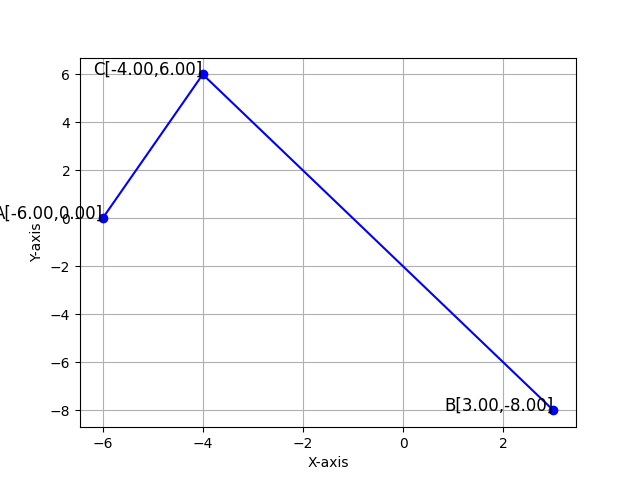
\includegraphics[width=0.7\linewidth]{figs/plot.png}
   \caption{ }
   \label{stemplot}
\end{figure}\\
\figref{stemplot} we can see that the given point doesn't lie on the line segment joining A and B.\\
\begin{align}
d_1&=\left\|{(A-C)}\right\|\\
\implies d_1^2&= (A-C)(A-C)^T\\
&=\myvec{
-2 & -6
}
\myvec{
-2\\
-6
}\\
\implies d_1&=\sqrt{40}\\
\end{align}
\begin{align}
d_2&=\left\|{(B-C)}\right\|\\
\implies d_2^2&=(B-C)(B-C)^T\\
&=\myvec{
7 & -14
}
\myvec{
7\\
-14
}\\
\implies d_2&=7\sqrt{5}\\
\therefore \frac{d_1}{d_2} &= \frac{\sqrt{40}}{7\sqrt{5}}
\end{align}
\begin{table}[h]
    \centering
    \begin{tabular}{|c|c|}
        \hline
        Point & Coordinates\\
        \hline
        $A$ & \myvec{0\\6}\\
        \hline
        $B$ & \myvec{8\\0}\\
        \hline
        $C$ & \myvec{0\\0}\\
        \hline
\end{tabular}

    \caption{Parameter Table}
    \label{tab.1}
\end{table}
\end{document}